\documentclass[a4paper]{article}
\usepackage[pdftex]{graphicx}
\usepackage[utf8]{inputenc}
\usepackage{enumerate}
\usepackage{siunitx}
\sisetup{locale=DE}
\usepackage{icomma}
\usepackage{amssymb}
\usepackage{tikz}
\usepackage{href-ul}
\hypersetup{
	colorlinks=true,
	linkcolor=blue,
	urlcolor=blue}
\usepackage{geometry}
\geometry{a4paper, top=15mm, left=15mm, right=15mm, bottom=15mm,
	headsep=10mm, footskip=12mm}

\begin{document}
	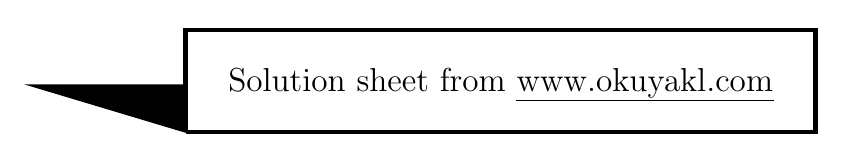
\begin{tikzpicture}(10,3)
		\draw[ultra thick](2,0) --(10,0) -- (10,1.3) --(2,1.3) -- (2,0);
		\draw[fill=black](2,0)-- (0,.6) -- (2,.6) -- (2,0);
		\node at (6,.6) {\large Solution sheet from \href{http://www.okuyakl.com}{www.okuyakl.com}};
	\end{tikzpicture}
	\vspace{0.5 cm}
	
	\noindent {\bf task 1. a)}\\
	The following applies to the angular velocity $\omega$:
	$$\omega = 2 \pi \cdot f = 2 \pi \cdot \SI{1.5}{\hertz}= \SI{9.4}{1\over\second}$$
	This is how the path speed is calculated:
	$$v_h = \omega \cdot r = \SI{9.4}{1\over\second} \cdot \SI{0.40}{\meter} = \SI{3.8}{\meter\over \second}$$
	\vspace{0.5 cm}
	
	\noindent {\bf task 1. b)}\\
	Horizontal throw: First we calculate the falling time of the ball. The following applies:
	$$
	\renewcommand{\arraystretch}{2}
	\begin{array}{rcl}
		h & = & {1\over 2}g\cdot t^2 \\
		t & = & \sqrt{2\cdot h \over g} \\
		t & = & \sqrt{2\cdot \SI{1.7}{\meter}\over \SI{9.81}{\meter\over {\second^2}}}\\
		t & = & \SI{0.59}{\second}
	\end{array}
	$$
	During this time she covered the distance in flight:
	$$ s = v_h \cdot t = \SI{3,8}{\meter\over \second} \cdot \SI{0.59}{\second} = \SI{2,2}{\meter}$$
	So it hits the ground at a distance of $\SI{2,2}{\meter}$.
	\vspace{0.5 cm}
	
	\begin{minipage}{0.6\textwidth}
		We already know the speed $v_h$ as the horizontal speed. Now the falling speed $v_v= g \cdot t = \SI{5,8}{\meter\over \second}$ is added as a further vertical component.
		Both velocity vectors form a right-angled triangle
		$$\tan{\alpha}= {v_v \over v_h} \quad \Leftrightarrow \quad \alpha = \tan^{-1} \left({\SI{5,8}{\meter\over \second} \over \SI{3,8}{\meter\over \second}}\right) = \SI{57}{\degree}$$
	\end{minipage}
	\hspace{0.5 cm}
	\begin{minipage}{0.3\textwidth}
		\setlength{\unitlength}{1.5 cm}
		\begin{picture}(3,2)
			\put(0,2){\vector(0,-1){2}}
			\put(0,0){\vector(1,0){3}}
			\put(0,2){\vector(3,-2){3}}
			\put(0.1,1){${v_v}$}
			\put(1.3,0.2){${v_h}$}
			\put(1.8,1){${v_{ges}}$}
			\put(2.4,0.1){$\alpha$}
		\end{picture}
	\end{minipage}
	
	So the ball hits with the angle of $\SI{57}{\degree}$.
	\vspace{0.5 cm}
	
	\noindent{\bf Task 2.}\\
	Its speed is $v=\SI{10}{\meter\over \second}$; the radius is $r=14\cdot \SI{2.5}{\centi\meter}= \SI{0.35}{\meter}$.
	So the frequency at which the wheels turn is:
	$$ f = {v \over 2\pi r} = {\SI{10}{\meter\over \second} \over 2 \pi \cdot \SI{0.35}{\meter}}=\SI {4.5}{\hertz}$$
	\vspace{0.5 cm}
	
	\noindent{\bf Task 3. a)}\\
	It applies to the speeds $v_i$ (inside) and $v_a$ (outside) of the read head and thus to $f_i$ and $f_a$:
	$$
	\renewcommand{\arraystretch}{2}
	\begin{array}{rclll}
		v_i &=& v_a \\
		2\pi f_i \cdot r_i &=& 2\pi f_a \cdot r_a\\
		f_i \cdot r_i &=& f_a \cdot r_a\\
		f_a &=& f_i \cdot {r_i \over r_a} &= \SI{500}{1\over\min} \cdot {\SI{2,2}{\centi\meter} \over \SI{5, 8}{\centi\meter}}&=\SI{190}{1\over\min}
	\end{array}
	$$
	We can calculate in the given units because this is a pure ratio equation.
	\vspace{0.5 cm}
	
	\noindent{\bf Task 3. b)}\\
	For estimation we calculate with the mean values $\bar{f}\approx \SI{350}{1\over\min}$; $\bar{r}\approx \SI{4}{\centi\meter}$.
	So the length of the track is:
	$$l = v\cdot t = 2\pi \bar{f} \cdot \bar{r} \cdot t = 2 \pi \cdot {350\over \SI{60}{\second}} \cdot \SI{0.04}{\meter} \cdot 74\cdot \SI{60}{\second} = \SI{6509}{\meter} \approx \SI{6.5}{\kilo\meter}$$
	\vspace{0.5 cm}
	
	\noindent{\bf Task 3. c)}\\
	The area of the recordable ring of the CD is:
	$$A=(r_a^2-r_i^2)\cdot \pi =\SI{90}{\centi\meter^2}$$
	Width of the track = area divided by length of the track:
	$$b={A \over l} = {\SI{0.009}{\meter^2} \over \SI{6509}{\meter}} \approx \SI{1.4e-7}{\meter} =\SI{140}{\nano\meter}$$
	\vspace{0.5 cm}
	
	\noindent{\bf Task 4.}\\
	The tire speed is one third of the engine speed; the speed is then:
	$$v = \omega r = 2\pi f \cdot r = 2\pi \cdot {4500 \over 3 \cdot \SI{60}{\second} }\cdot \SI{0.30}{\meter } =\SI{47}{\meter\over \second}\approx \SI{170}{\kilo\meter\over \hour}$$
	\vspace{0.5 cm}
	
	\noindent{\bf Task 5.}\\
	One full revolution corresponds to one hour, the circumference is:
	$$U=2\pi r = 2 \pi \cdot \SI{3}{\meter} \approx \SI{19}{\meter}$$
	One minute equals one-sixtieth of it:
	$$b_{1min} = {\SI{19}{\meter} \over 60}=\SI{30}{\centi\meter}$$
	Analogously, one second corresponds to:
	$$b_{1s}= {\SI{19}{\meter} \over 3600}=\SI{5}{\milli\meter}$$
	\vspace{0.5 cm}
	
	\noindent{\bf Task 6.}\\
	It applies again to the speed:
	$$v=\omega r = 2 \pi f \cdot R = {2 \pi \over T} \cdot R = {{}2\pi \over 24 \cdot 60 \cdot \SI{60}{\second}} \cdot \SI{6378e3}{\meter} = \SI{463}{\meter\over\second}$$
	\vspace{0.5 cm}
	
	\noindent{\bf Task 7.}\\
	$$r = {v \over \omega} ={v \over 2\pi f}= {\SI{2,2e6}{\meter\over\second} \over 2 \pi \cdot \SI{6, 6e15}{1\over\second}}= \SI{5,3e-11}{\meter}$$
	\vspace{0.5 cm}
	
	\noindent{\bf Task 8.}\\
	\renewcommand{\arraystretch}{2}
	\begin{tabular}{|c|c|c|c|c|c|c|c|c|}
		\hline
		Body & Mercury & Venus & Earth & Mars & Jupiter & Saturn & Uranus & Neptune \\
		\hline
		mean solar distance in $\SI{1e6}{\kilo\meter}$ & 57.9 & 108.2 & 149.6 & 227.9 & 778.3 & 1427 & 2871 & 4498\\
		\hline
		Orbital period in a & 0.241 & 0.615 & 1.000 & 1.881 &11.86 &29.45 & 84.02 & 164.8\\
		\hline
		average path speed in $\SI{}{\kilo\meter\over \second}$ & 47.9 & 35.1 & 29.8 & 24.1 & 13.1& 9.65 & 6.80 & 5.43 \\
		\hline
	\end{tabular}
	\vspace{0.5 cm}
	
	\noindent{\bf Task 9. a)}\\
	The following applies to the conversion from degrees to radians:
	$${\alpha _{RAD} \over 2\pi} = {\alpha _{DEG} \over \SI{360}{\degree}} \quad \Rightarrow \quad
	\alpha _{RAD}={\alpha _{DEG} \over \SI{360}{\degree}}\cdot 2\pi = {\SI{0.0040}{\degree} \over \SI{360}{ \degree}} \cdot 2 \pi = 7.0 \cdot 10^{-5}$$
	But the mirror has only rotated further by half the angle, so $\alpha= 3.5\cdot 10^{-5}$.
	\vspace{0.5 cm}
	
	\noindent{\bf Task 9. b)}\\
	The angle of rotation is the angular velocity multiplied by time. This means that the light travel time is:
	$$ \alpha = \omega \cdot t \quad \Rightarrow \quad t = {\alpha \over \omega}={3.5 \cdot 10^{-5} \over 2\cdot \pi \cdot \SI {100}{1\over\second}}=\SI{5,6e-8}{\second}$$
	This makes it easy to calculate $c$:
	$$c={2\cdot d \over t}={2\cdot \SI{8,0}{\meter} \over \SI{5,6e-8}{\second}}=\SI{2 ,9e8}{\meter\over\second}$$
	\vspace{0.5 cm}
	
	\begin{center}
		\includegraphics[width=7 cm]{../../viecher/eendcomic.pdf}
		
		Here you can go back to the \href{https://www.okuyakl.de/phys/p10kreaL414/ae414.pdf}{task sheet}
	\end{center}
	
	\end{document}